La especificación de requisitos de usuario pretende recoger las necesidades de
los usuarios finales del producto para tenerlas en cuenta a lo largo del desarrollo
del mismo.

Para esta labor, se ha realizado un cuestionario voluntario donde la comunidad de
conductores y no conductores informaban de sus preferencias, gustos, necesidades y
otra información que se pudiera considerar relevante.

Como los encuestados se mezclaban, se ha decidido hacer una separación por
conductores y no conductores teniendo en cuenta sus preferencias. La distribución
de las preguntas quedaba de esta forma:

\begin{enumerate}
  \item Se le pregunta al encuestado datos básicos y si es conductor.
  \item En caso afirmativo, se recoge esta información:
        \begin{itemize}
          \item Años de carnet.
          \item Tipo de carnet.
          \item Edad del conductor.
          \item Tecnologías que presenta el vehículo de uso habitual.
          \item Tipo de vehículo de uso habitual.
          \item Años del vehículo de uso habitual.
        \end{itemize}
  \item A continuación, se le muestra al usuario una matriz de selección en donde,
        de una escala del 1 al 20, debe priorizar los distintos elementos que aparecen
        (en total, 20). Solo se permite una única prioridad por elemento, de forma que
        múltiples elementos tengan la misma prioridad.

        Los elementos que se han propuesto en este cuestionario son (tabla \ref{tab:options}):

        \begin{table}[H]
          \centering
          \begin{tabularx}{\textwidth}{| C{.25} | C{.25} | C{.25}| C{.25} |}
            \hline
            Visualización en tiempo real   & Información detallada de errores & Velocímetro                  & Cuentarrevoluciones                        \\
            \hline
            Marcha actual (1ª, 2ª, \dots)  & Temperatura del aceite           & Presión del aceite           & Temperatura exterior                       \\
            \hline
            Intensidad del acelerador (\%) & Consumo actual                   & Presión de las ruedas        & Presión de los inyectores                  \\
            \hline
            Nivel de combustible           & Distancia recorrida              & Nivel de batería             & Nivel de carga en valor absoluto del motor \\
            \hline
            Presión atmosférica            & Temperatura de la toma de aire   & Temperatura del refrigerante & Temperatura del motor                      \\
            \hline
          \end{tabularx}
          \caption{Opciones ofrecidas a los encuestados. Se han escogido diversas opciones que se encuentran entre los datos habituales generados por un vehículo.}
          \label{tab:options}
        \end{table}
  \item Finalmente, de forma libre, se le pide al usuario que indique qué sensores
        añadiría a su vehículo (si tiene), qué datos querría poder medir y qué
        tareas querría automatizar.
\end{enumerate}

Las opciones anteriores se componen de elementos que se pueden obtener mediante el
\ac{OBD} estándar, usando una lista de \textit{pids} comunes públicos que
todos los vehículos deberían usar \cite{OBDIIPIDs2021}. Dado que la encuesta se
podía realizar tanto por conductores como por no conductores, se van a separar las
respuestas en donde se evaluará la población global (tabla \ref{tab:global}) y
luego a la población únicamente de conductores (tabla \ref{tab:drivers}).
Todo el desglose y el análisis se encuentra disponible en:
\url{https://s.javinator9889.com/vims-analysis}.

\begin{table}[H]
  \centering
  \begin{minipage}{.48\linewidth}
    \begin{tabularx}{\textwidth}{|C{.3}|C{.7}|}
      \hline
      \textbf{Puntuación} & \textbf{Opción}                            \\
      \hline
      1                   & Velocímetro                                \\
      1                   & Nivel de combustible                       \\
      4                   & Marcha actual                              \\
      5                   & Distancia recorrida                        \\
      5                   & Nivel de batería                           \\
      6                   & Cuentarrevoluciones                        \\
      8                   & Intensidad del acelerador (\%)             \\
      8                   & Presión de las ruedas                      \\
      10                  & Temperatura del aceite                     \\
      10                  & Nivel de carga en valor absoluto del motor \\
      12                  & Visionado en tiempo real                   \\
      12                  & Consumo actual                             \\
      12                  & Temperatura del motor                      \\
      14                  & Presión del aceite                         \\
      14                  & Temperatura del refrigerante               \\
      16                  & Presión atmosférica                        \\
      17                  & Temperatura exterior                       \\
      19                  & Información detallada de errores           \\
      19                  & Presión de los inyectores                  \\
      20                  & Temperatura de la toma de aire             \\
      \hline
    \end{tabularx}
    \caption{Puntuaciones obtenidas de forma general, por la población al completo (conductores y no conductores).}
    \label{tab:global}
  \end{minipage}
  \hfill
  \begin{minipage}{.48\linewidth}
    \begin{tabularx}{\textwidth}{|C{.3}|C{.7}|}
      \hline
      \textbf{Puntuación} & \textbf{Opción}                   \\
      \hline
      1                   & Velocímetro                       \\
      1                   & Nivel de combustible              \\
      3                   & Temperatura del motor             \\
      4                   & Temperatura del aceite            \\
      4                   & Nivel de batería                  \\
      5                   & Distancia recorrida               \\
      6                   & Cuentarrevoluciones               \\
      7                   & Presión de los inyectores         \\
      8                   & Presión de las ruedas             \\
      10                  & Presión del aceite                \\
      11                  & Marcha actual                     \\
      11                  & Presión atmosférica               \\
      14                  & Temperatura del refrigerante      \\
      15                  & Temperatura exterior              \\
      17                  & Intensidad del acelerador (\%)    \\
      18                  & Información detallada de errores  \\
      18                  & Consumo actual                    \\
      19                  & Temperatura de la toma de aire    \\
      20                  & Visionado en tiempo real          \\
      20                  & Nivel de carga absoluta del motor \\
      \hline
    \end{tabularx}
    \caption{Puntuaciones obtenidas de forma general, por la población (excluídos los no conductores).}
    \label{tab:drivers}
  \end{minipage}
\end{table}

Resulta interesante ver cómo varios elementos coinciden en puntuación y posición, como
el \textit{Velocímetro} o el \textit{Nivel de combustible} mientras que otros se
mueven radicalmente de posición, como la \textit{Marcha actual}, la \textit{Temperatura 
del motor}, etc.

En general, se observa cómo los usuarios quieren tener más información sobre distintos
elementos del vehículo y no necesariamente en ``tiempo real'' sino \textit{a posteriori},
como información estadística. En particular, entre la comunidad de conductores prima
información mecánica y relativa al estado del vehículo más allá de información sobre
el viaje.

Además, hay bastante interés en la automatización de ciertas acciones como el cierre
de las puertas automáticamente, \textit{reset} del odómetro cuando se repuesta, 
notificaciones cuando haya que realizar labores de mantenimiento, etc. Sin embargo,
el diseño inicial del proyecto no contempla el realizar acciones sobre el automóvil
principalmente porque los conectores estándar permiten la lectura de
datos pero no la escritura. Para conseguir enviar información al vehículo sería
necesario realizar un montaje directamente sobre los cables de los buses \ac{CAN} que
tiene, escuchar de forma activa las tramas y generar la información a enviar.
En principio, esto se encuentra fuera del alcance del proyecto, por lo que se
ignoran todas las modificaciones sobre el automóvil en sí.

Finalmente, se observa que hay un interés generalizado en que la interfaz sea
simple, en que se pueda saber dónde se ha aparcado el vehículo y
en que el sistema sea fluido y rápido.

A partir de lo anterior, se definen los siguientes requisitos de usuario:

\begin{enumerate}[label=\textbf{\texttt{RU-\arabic*}}]
  \item\label{ru:rt} Como usuario no necesito que la información se muestre en tiempo
        real sino que se almacene para una posterior consulta, o bien en forma de
        estadísticas o bien como datos en crudo. Dichas estadísticas se conformarían
        de la media, varianza, tendencia y moda de los datos de interés recogidos individualmente
        por cada conductor durante el uso del vehículo, destacando la velocidad,
        carga del motor, consumo, tiempo acelerando, metros ascendidos, metros descendidos,
        etc.
  \item\label{ru:status} Como conductor me gustaría conocer de primera mano el estado
        del motor, a niveles tanto de temperatura de los elementos principales como
        de estado de los distintos elementos mecánicos del mismo.
  \item\label{ru:maintenance} Como usuario, me gustaría conocer fácilmente
        información relativa al mantenimiento del vehículo, como el desgaste de
        las ruedas, nivel de aceite, líquido de frenos, etc.
  \item\label{ru:notifications} Como usuario, y en estrecha relación con
        \ref{ru:maintenance}, me gustaría recibir una notificación o alerta sobre
        cuándo se debe realizar el mantenimiento del vehículo. 
  \item\label{ru:err-notifications} Como usuario también querría ser notificado si se detecta algún error o problema
        en el vehículo.
  \item\label{ru:parking} Como conductor, me gustaría saber dónde he aparcado el
        vehículo.
  \item\label{ru:stats} Como conductor, me gustaría que tras realizar un viaje
        o tras realizar un repostaje se generasen estadísticas que me sirviesen para
        analizar mi perfil de conducción.
  \item\label{ru:recommendations} Como usuario, me gustaría recibir recomendaciones
        sobre mi estilo de conducción para optimizar el consumo o entender mejor cómo
        manejar el vehículo.
  \item\label{ru:speed} Como usuario, me gustaría que el sistema fuese fluido y
        funcionase bien, con tiempos de carga pequeños y sin ir a trompicones.
  \item\label{ru:intuitive} Como usuario, me gustaría que el sistema fuese accesible
        e intuitivo, simple a primera vista pero personalizable.
        Se propone una interfaz como la que se muestra en la figura \ref{fig:data-ui}
        que permite seleccionar el rango temporal sobre el cual evaluar los datos
        y la información estadística definida en \ref{ru:rt}:

        \begin{figure}[H]
            \centering
            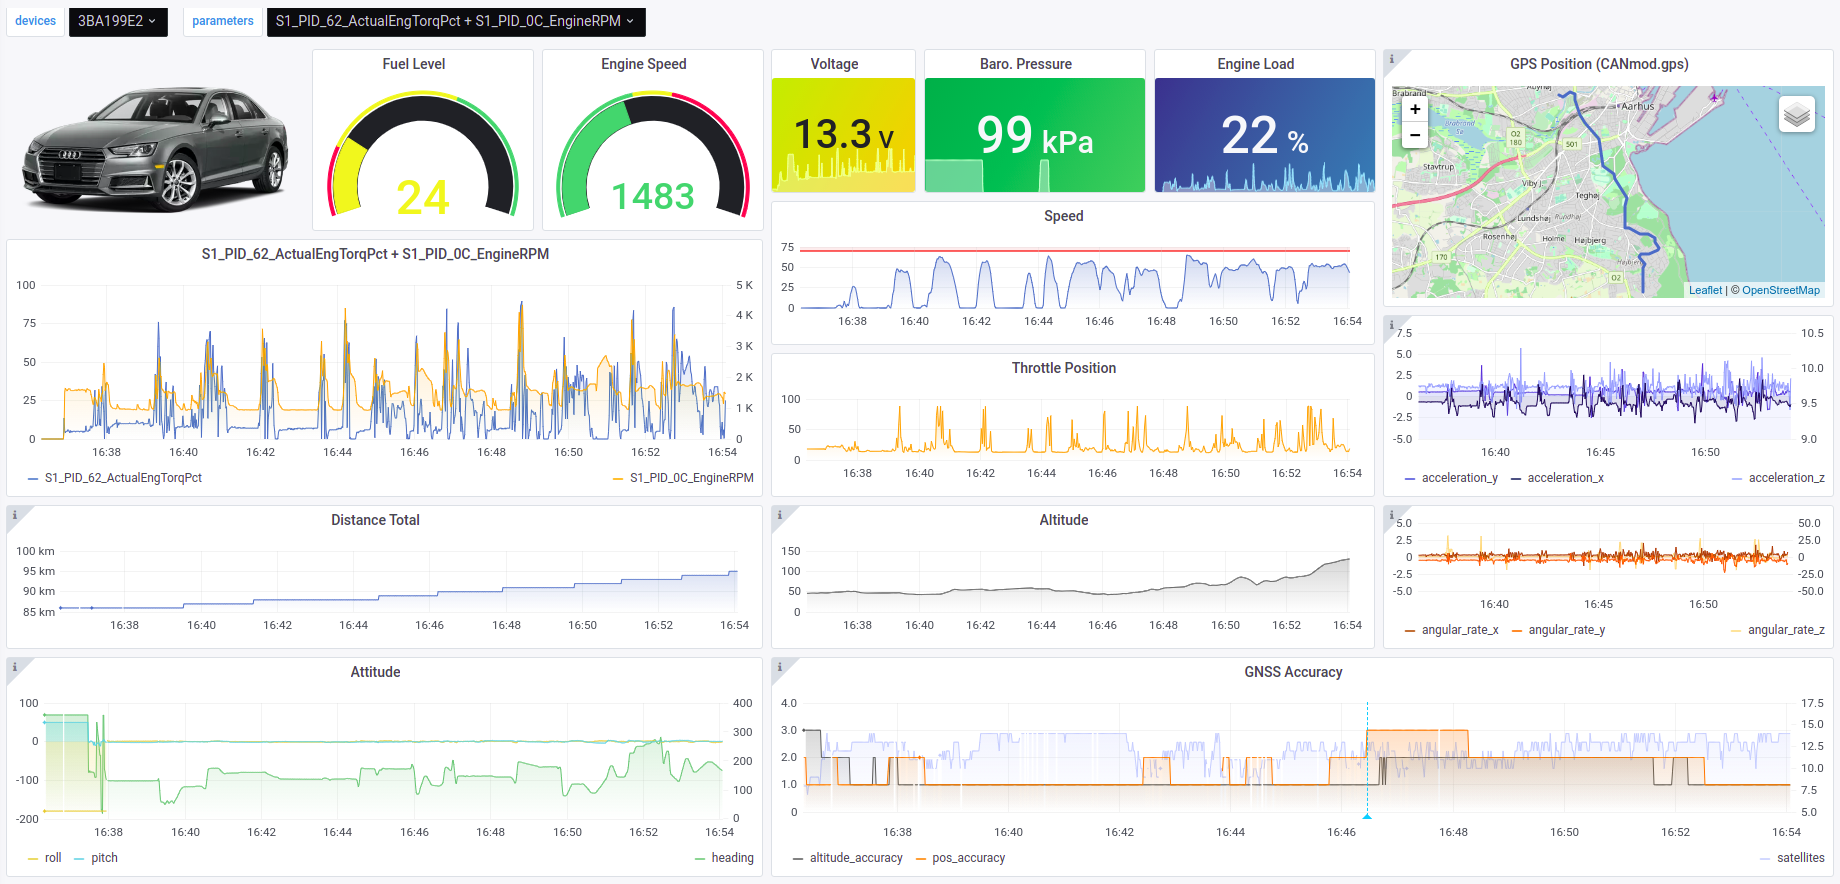
\includegraphics[width=\linewidth]{images/data-ui.png}
            \caption{Representación de los datos en la interfaz propuesta -- fuente: \url{https://grafana.csselectronics.stellarhosted.com/d/6qvL9OvMz/css-playground-obd2?orgId=1}.}
            \label{fig:data-ui}
        \end{figure}
\end{enumerate}